\chapter{The newTRENDs Project} 

The aim of NewTRENDs is to increase the qualitative and quantitative understanding of impacts of New Societal Trends on energy consumption and to improve the modelling of energy demand, energy efficiency and policy instruments \cite{fraunhofer}. 

\section{Concept}

%The newTRENDs project develops the analytical basis for a ``2050 Energy Efficiency Vision" by considering New Societal Trends in energy demand modeling \cite{newtrends}.

With increasing renewable generation integrated into the power system, supply-side fluctuations must be balanced by demand-side flexibility. 
Electrification and demand response (DR) are becoming increasingly relevant to the heating transition of buildings, which demands the diffusion of

\begin{itemize}
  \item heat pumps (HPs),
  \item photovoltaic (PV) and energy storage (e.g., battery and hot water tank),
  \item smart energy management systems (SEMSs).
\end{itemize}

Combining the three technologies is also beneficial from an individual household (or building) perspective. The household can optimize the heat pump operation to reduce energy costs by saving energy in the tanks or pre-heat the building when the electricity price is lower. Besides, the energy-saving benefit could be further increased with PV and battery system.
From a market perspective, DR flexibility and PV generation also facilitate the concept of "energy community". The households can trade electricity with each other (peer-to-peer, P2P) within a local micro-grid or even trade with the other side of the country through the national grid, depending on the infrastructure, business model, and policies. In addition, households can also buy the services from an "aggregator", who bundles and manages the flexibility of small consumers and producers and participate in the market activities (Kerscher and Arboleya 2022). 
Promoted by the declining costs of technologies and support policies, more and more household "consumers" are expected to become "prosumers" (with PV) and "prosumagers" (plus energy storage and SEMS) (Fereidoon Sioshansi 2019).

\section{FLEX models}

The FLEX-Operation and FLEX-Community models were built to improve the building modeling suite and to analyze the societal trends of prosumaging and energy communities.
The figure below shows how FLEX interacts with other bottom-up models involved in the newTRENDs project.

\begin{figure}[h]
  \centering
  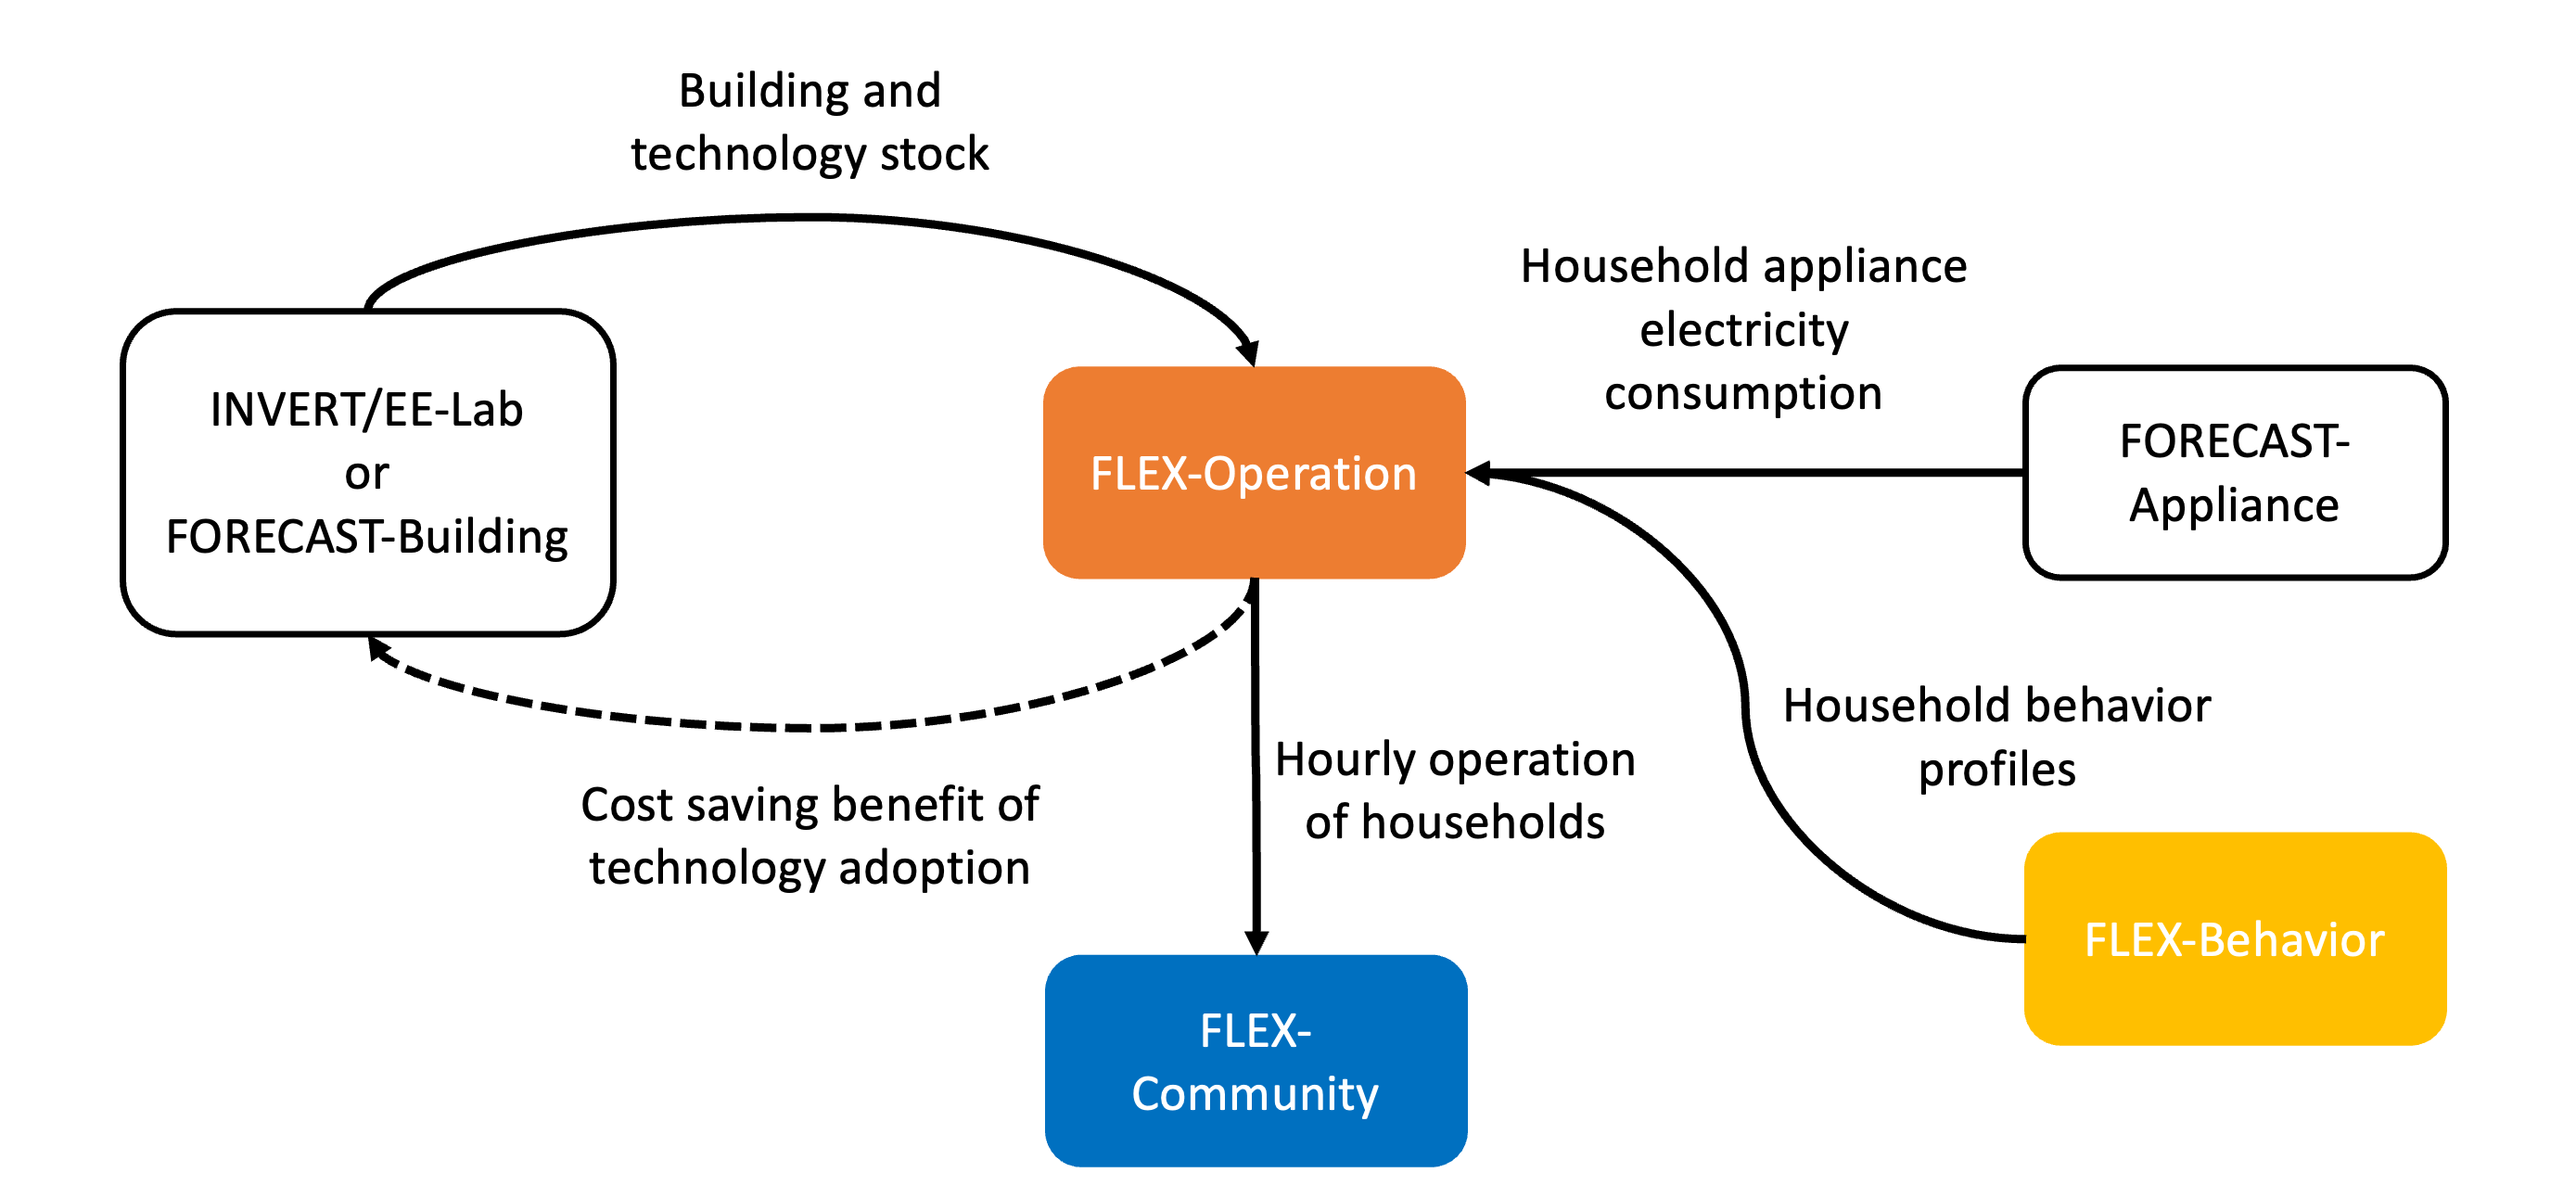
\includegraphics[width=\textwidth]{Images/flex.png}
  \caption{FLEX}
\end{figure}

\subsection{FLEX-Operation}

FLEX-Operation models the energy system operation of an individual household in hourly resolution.  
It calculates the energy consumption of each representative building, including operation of technologies (e.g., battery, PV, heat pump, etc.) and load profiles in hourly resolution.

\subsection{FLEX-Community}

FLEX-Community models the operation of an energy community, i.e., household interaction, aggregator optimisation. 
It can be applied to support the aggregators designing and evaluating business models, as well as making investment decisions, for example, the self-owned battery, PV panels, etc.

\subsection{FLEX-Behavior}

FLEX-Behavior models the behavior (activity profile) of households' and corresponding load profiles. 
It generates the hourly activity and energy demand profile of a pre-defined individual household. 
The results include

\begin{enumerate}
  \item appliance electricity demand,
  \item domestic hot water demand,
  \item driving profile, and
  \item building occupation.
\end{enumerate}

Data will be considered by the model is

\begin{itemize}
  \item building,
  \item heating system (heat pump, fuel-based boiler, electric heater),
  \item thermal storages for space heating and domestic hot water,
  \item space cooling technology,
  \item PV,
  \item battery, and
  \item electric vehicle.
\end{itemize}

This proposed thesis is going to focus on FLEX-Behavior model. 

\section{Motivations}

This would be an opportunity to encourage European households, that are under suitable conditions, to switch to greener energy options. 
That actually do benefits for not only the environment but also for the planet. 

\section{Research gaps and questions}

There is a lack of research and design case studies to promote energy optimisation solutions from a user's perspective. 
This proposed thesis will unfold from following perspectives

\begin{itemize}
  \item Awareness and understanding of new energy sources
  \item Demand for new energy sources
  \item Confidence in new energy solutions
  \item Feasibility of adopting new energy options
\end{itemize}

The aims of the proposed thesis are 
\textit{(i)} implementation of proposed smart energy optimisation recommender as a web application, using data visualisation techniques designed for different types of households. 
\textit{(ii)} evaluation of the explainability of smart energy optimisation recommender at the user level and measuring the impact of the households perceptions towards energy optimisation solutions. 
\textit{(iii)} provide a design guideline on how to enable trust in energy optimisation solutions when trying to promote green energy plans. 

\begin{itemize}
  \item Building typical household profiles.
  \item A decision tree is used to obtain information about the user by analys\-ing the profiles and predicting them in order to reduce the number of steps involved in entering user data.
  \item The result is an interpretable energy optimisation solution.
\end{itemize}

